\label{chapter: introduction}

These are lecture notes from the Active Matter course held in the summer semester of 2024 at the University of Göttingen.
The lectures are by Benoît Mahault and Ramin Golestanian of the Max Planck Insitute of Dynamics and Self-Organization, featuring a range of guest lecturers, and the notes are typeset by Martin Kjøllesdal Johnsrud.
The notes meant to give a short introduction to the field of Active Matter Physics, and present some background material in the form of concepts and mathematical tools used to study active systems.

% Handwritten page I 


\subsection{What is active matter?}

\todo[inline]{Re-draw figures}

As widely accepted definition of active matter consists to say that it is made of elementary units that locally dissipate energy in a continuous and sustained manner. Hence, the dynamics of active particles break time-reversal symmetry, \textit{it is inherently far from thermodynamic equilibrium}. In many cases, activity manifests as persistent motion, but can also take the form of local production of forces, sustaining of chemical reactions, growth (reproduction), or several of them at the same time. This definition is very broad and encompasses a multitude of biological examples spanning many scales:

\begin{figure}[!htb]
    \centering
    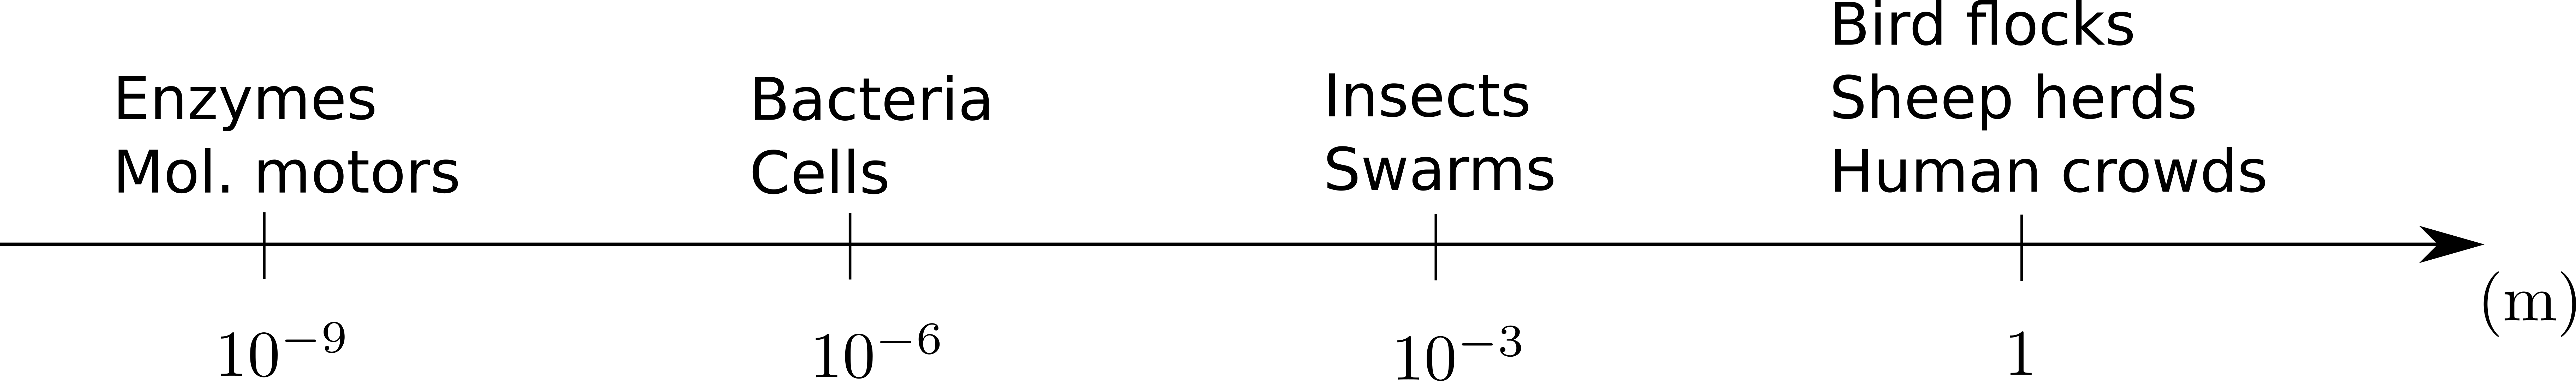
\includegraphics[width=.8\textwidth]{Figures/introduction/scales.png}
    \caption{The range of scales of active particles.}
    \label{fig: scales active particles}
\end{figure}


% Handwritten page II
Some examples of active systems are:

\begin{itemize}
    \item Enzymes, molecular motors (nm): Enzymes (E) catalyze chemical reactions of a substrate (S),
    %
    \begin{align}
        E + S \longrightarrow  \underbrace{SE}_{\mathrm{binding}} \longrightarrow  E + P
    \end{align}
    %
     and thus locally generate chemical gradients, $\bm \nabla P$. 
     \begin{figure}[H]
        \centering
        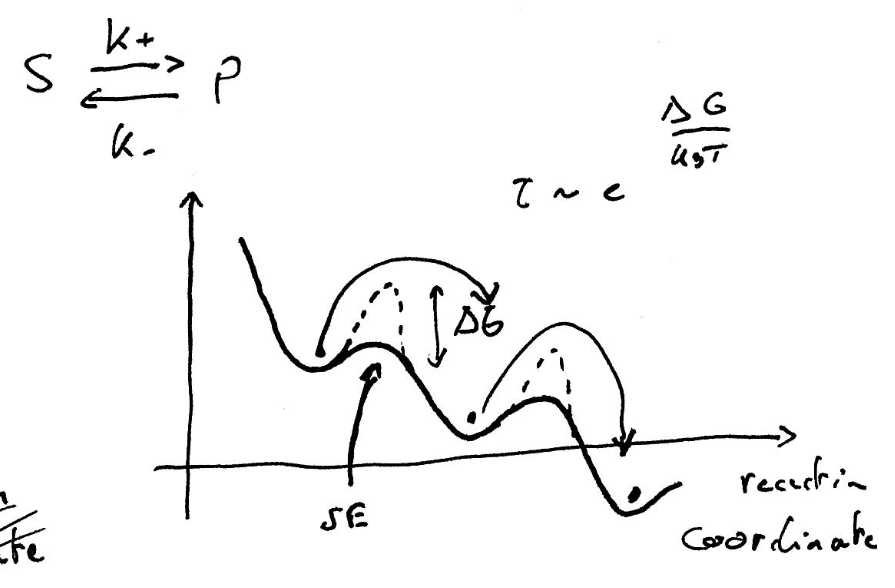
\includegraphics[width=.3\textwidth]{Figures/introduction/enzymes.png}
        \caption{The energy landscape for the chemical reaction is modified by the }
        \label{fig: enzymes}
    \end{figure}
     Molecular motors couple chemical cycles to displacements or rotations, so that these molecular machines can exhibit self-propulsion.\\
     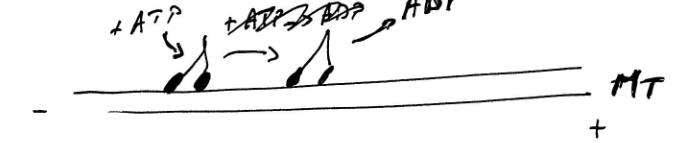
\includegraphics[width=.3\textwidth]{Figures/introduction/motors.png}
    \item Bacteria, cells ($\mu$m): Bacteria and algae usually move thanks to filamentous appendices called flagella or cilia, which are powered by molecular motors.
    \\
    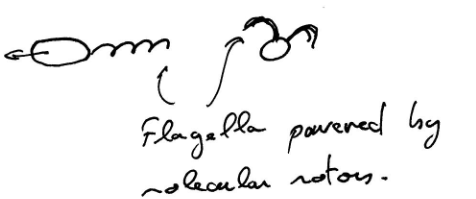
\includegraphics[width=.3\textwidth]{Figures/introduction/bacteria.png} 
    \\
    Another example is cells that self-propel on the substrate by polymerizing actin filaments at their front.
    \\
    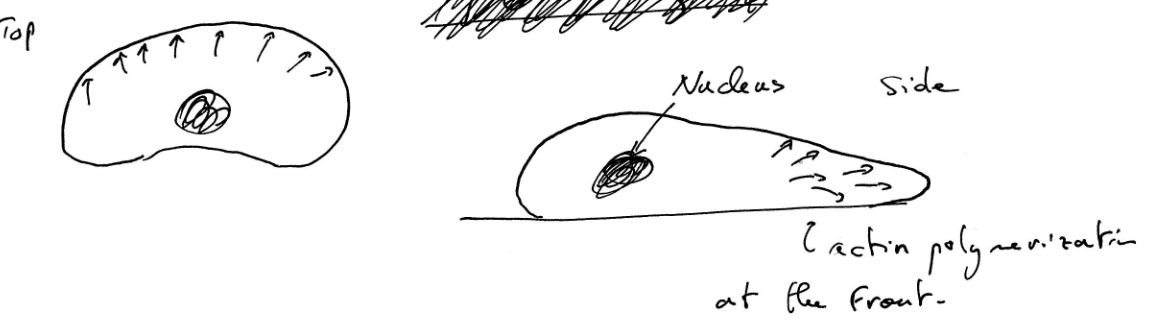
\includegraphics[width=.25\textwidth]{Figures/introduction/actin.png}
    \item Insect swarms (mm)
    \item Animal herds, human crowds (m)
\end{itemize}


% Handwritten page III

\subsection{What makes active matter special?}

Active systems, because they constantly dissipate energy in their bulk, and in contrast to passive systems globally driven (turbulence, shaken granulars, \ldots), are able to spontaneously self-organize and create macroscopic structures. 
Again, these ideas are relevant to many examples in the living world including the architecture of the cytoskeleton, the morphogenesis of multicellular organisms, or the collective motion arising from social interactions in groups of several hundred or thousands of individuals. 

Active matter is also not restricted to the study of biological systems, as the design and study of synthetic active particles now represent a large part of the field. Those allow for better controlled experiments and often exhibit similar phenomenology as their biological counterpart, thus opening the way to biomimetic materials engineering. 
\todo[noinline]{Notorious? isn't that a bit negative?}
Notorious examples of artificial active matter include assemblies of self-propelled colloids (Phoretic Janus particles, Quincke rollers), artificial microswimmers (self-propelled drops, magnetic swimmers), and robots.\todo[noinline]{Give ref}

\begin{figure}[!htb]
    \centering
    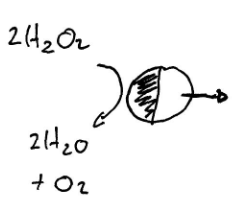
\includegraphics[width=.3\textwidth]{Figures/introduction/janus.png}
    \caption{A self-propelled Janus particle, to be discussed in Lecture 7}
    \label{fig: janus}
\end{figure}



\subsection{On the nonequilibriumness of active assemblies}

As written above, active matter is inherently `far' from equilibrium, since it is assembled from particles whose dynamics constantly break time-reversal symmetry. This means that active systems lack many of the properties familiar to equilibrium systems. These include:
%
\begin{enumerate}
    \item Absence of minimization principle: active dynamics are not constrained by the second law, so that they do not converge over long times to a state with maximal entropy (or minimum free energy). In fact, whether an active system converges to a steady state or not is a priori unknown.
    \item No time-reversal symmetry: as a consequence of 1, active systems can (and do) generally produce macroscopic currents, leading to phases where TRS is collectively broken.
    \item Lack of thermodynamic framework: Basic equilibrium concepts such as temperature or thermodynamic pressure are usually not defined for active systems. Additionally, active systems generally do not exhibit an equation of state, meaning that their bulk properties are not only determined by their material properties but can also be substantially affected by the nature and shape of the container they live in.
    \item Memory: again, due to 1 and contrary to systems at equilibrium, the state of an active system may be dependent of its past history.
    \item In active matter, momentum is not conserved so forces do not necessarily need to satisfy the action-reaction principle. Familiar examples of such `nonreciprocity' are encountered in predator-prey systems, while it also generally arises when particles interact via self-generated fields such as bacteria or phoretic colloids.
\end{enumerate}
%
In summary, the collective behaviors found in active systems thus generally break our intuition built on equilibrium physics, and their theoretical understanding requires to use and develop specifically tailored tools and concepts.
In particular, we will construct field theory descriptions of active systems, such as irreversible thermodynamics and perform coarse-graining using kinetic theory.\todo[noinline]{Is this right?}


% Handwritten Page IV

\subsection{The idea of this course}

Active matter is very large and quickly developing field borrowing tools and concepts from various other areas of physics including soft matter, biological physics, hydrodynamics, and statistical physics. So, this course is only meant as an introduction to the basics of the very diverse phenomenology of active systems, and how it is usually apprehended. In particular, our journey will be driven by two general aspects which are still the topic of active research:
\begin{itemize}
    \item How is active motion generated at the micro scale, and what are its consequences on the dynamics of active particles?
    \item How do active systems convert energy dissipated at the molecular scale into the formation of structure and order macroscopic scales?
\end{itemize}
These two lectures is meant to give an overview of the topic that will be addressed in the following weeks, while we will also introduce useful concepts and mathematical tools.



% Handwritten page V

\section{Hydrodynamics of microswimmers}

Many active particles evolve in a fluid, which they need to displace in order to move. Understanding the locomotion of such swimmers thus requires to study the dynamics of the flow around them. The fluid surrounding the particles is generally incompressible so that it is defined by its local velocity $\bm v$ which obeys the Navier-Stokes equations:
%
\begin{subequations}
\label{eq_NS}
\begin{align}
    \label{eq_NS_v}
    \rho \left[ \partial_t \bm v + (\bm v \cdot \nabla)\bm v \right] & = \eta \nabla^2\bm v - \nabla P + \bm f, \\
    \label{eq_NS_inc}
    \nabla \cdot \bm v & = 0.
\end{align}
\end{subequations}
%
The terms on the left-hand side of~\eqref{eq_NS_v} correspond to the material derivative and simply model the effect of inertia, while on the right-hand side the first term originates from viscous dissipation, the second is the pressure which ensures incompressibility as required by~\eqref{eq_NS_inc}, while the active force $\bm f$ arises as a source term.
In cases dominated by inertia or dissipation, the NS Eq.~\eqref{eq_NS} simplifies. To understand this, let us define the typical length and velocity scales of the problem, $L$ and $V$, and apply the following rescaling:
%
\begin{equation*}
    \bm v \to V \bm v', \quad
    \bm x \to L \bm x', \quad
    t \to \frac{L}{V}t', \quad
    P \to \frac{\eta V}{L} P', \quad
    \bm f \to \frac{\eta V}{L^2} \bm f'.
\end{equation*}
%
We obtain the following equation in terms of the dimensionless primed variables
%
\begin{equation}
    {\rm Re}\left[ \partial_{t'} \bm v' + (\bm v' \cdot \nabla')\bm v' \right] = \nabla'^2\bm v' - \nabla' P' + \bm f',
\end{equation}
%
where ${\rm Re} = \rho V L / \eta$ is known as the Reynolds number. 
Alternatively, note that the Reynolds number can be obtained by the ratio of the typical scales associated with the convection ($\bm v\cdot \nabla \bm v$) and dissipation ($\eta\nabla^2\bm v$) in the Navier-Stokes equation. 
Hence, the value of the Reynolds number controls the relative importance of inertial effects and viscous dissipation.
For a micron-sized swimmer in water such as bacteria, we can evaluate $\rho \approx 10^3 \; {\rm kg / m^3}$, $\eta \approx 10^{-3} \; {\rm Pa \cdot s}$,
$V \approx 10^{-5}\; {\rm m/s}$, and $L \approx 10^{-6} \; {\rm m}$, such that ${\rm Re} \approx 10^{-5}$.
%
% Handwritten page VI
%
\textit{Microswimmers therefore evolve at vanishing Reynolds number} where inertial effects are negligible. 
Their dynamics then evolve in the so-called Stokes regime, 
such that the flow they generate obeys the Stokes equation:
%
\begin{subequations}
\label{eq_Stokes}
\begin{align}
    \label{eq_Stokes_v}
    \eta \nabla^2\bm v -\nabla P + \bm f & = \bm 0, \\
    \label{eq_Stokes_inc}
    \nabla \cdot \bm v & = 0.
\end{align}
\end{subequations}
%
Contrary to the Navier-Stokes equation, Eqs.~\eqref{eq_Stokes} do not have time derivatives and are linear.
The flow velocity $\bm v$ only therefore only depends on the instantaneous value of the force $\bm f$ (there is no inertia), and it varies linearly with it\footnote{By taking the divergence of~\eqref{eq_Stokes_v}, you can convince yourself that the pressure is also a linear function of the force.}. 
An important consequence of these features is that is that Stokes flow obey kinematic reversibility, meaning that they obey the symmetry
%
\begin{equation*}
    \bm f \rightarrow -\bm f, \qquad \bm v \rightarrow -\bm v.
\end{equation*}
%
As such, sequences of motion are reversible.
One important consequence of this is the \emph{scallop theorem}, which states that a microswimmer cannot achieve self-propulsion with reciprocal motion.
%
\begin{figure}[!htb]
    \centering
    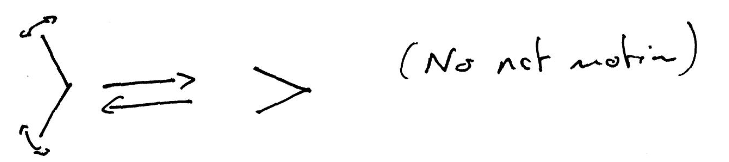
\includegraphics[width=.3\textwidth]{Figures/introduction/scallop.png}
    \caption{A scallop moves by opening and closing its shells, which in the Stokes regime gives zero net motion}
    \label{fig: scallop}
\end{figure}

The name comes from an example of reciprocal motion, a scallop opening and closing its shell
Self-propulsion therefore requires at least 2 independent degrees of freedom (d.o.f.)\todo[noinline]{I think this is not a good statement, unless dof is well defined}
Examples of this are swimmers with a corkscrew flagella or breast-stroke-like motion.
Such swimmers are force and torque-free, as the net forces/torques from the flagella and the drag adds up to zero.



\begin{figure}[!htb]
    \centering
    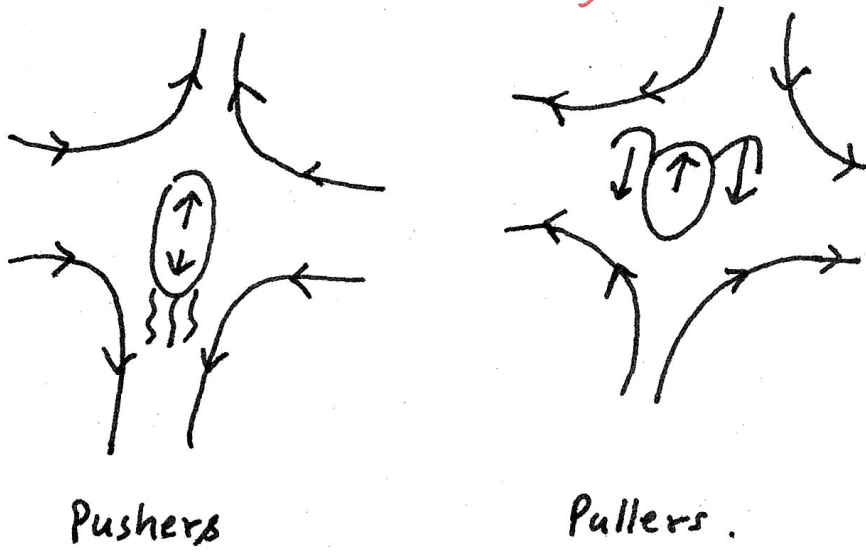
\includegraphics[width=.5\textwidth]{Figures/introduction/swimmers.png}
    \caption{Two examples of microswimmers}
    \label{fig: swimmers}
\end{figure}





% handwritten page VII

\section{A minimal model for active motion}


In the previous section, discussed by which mechanism active motion can arise (in the nontrivial context of microswimmers).
Here, we will be rather ask the question of what the consequences of the presence of a self-propulsion speed on the dynamics of an active particle are.
For this, assume that a particle is able to self-propel but we won't particularly focus on the details of its self-propulsion mechanism.


\subsection{Some basics on Brownian motion}

\begin{figure}[!htb]
    \centering
    \includegraphics[width=.25\textwidth]{Figures/introduction/brownian.png}
    \caption{A Brownian particle is constantly and randomly interacting with smaller particles.}
    \label{fig: brownian}
\end{figure}

Before discussing active motion, let us give a brief recap on the theory of Brownian motion.
Consider a micron-sized particle in a fluid at temperature $T$. 
The particle constantly undergoes collisions with the fluid molecules, and its mass is low enough that the results of such collisions result in visible erratic dynamics known as Brownian motion.
The dynamics of the particle is described by the \emph{Langevin equation}
%
\begin{equation} \label{eq_LangevinBM}
    m\frac{\rmd^2 \bm r}{\rmd t^2} + \zeta \frac{\rmd \bm r}{\rmd t} = \bm f(t).
\end{equation}
%
Equation~\eqref{eq_LangevinBM} is nothing but Newton's second law, so that the first term on the left hand side represents the acceleration of the particle multiplied by its mass, and the second term accounts for the Stokes friction exerted by the fluid in response to the motion of the particle.
In fact, the ratio of the particle mass and friction coefficient defines a timescale $\tau = m / \zeta$ beyond which inertial effects can be neglected.
For a micron-size sphere with a density comparable to that of water, we have
%
\begin{equation*}
    \tau = \frac{\rho \tfrac{4\pi}{3} R^3}{6 \pi \eta R} 
    = \frac{2\rho R^2}{9\eta} \approx 0.2 \; \mu{\rm s}.
\end{equation*}
%
Hence, for observation times beyond the micro-second inertial effects can generally be safely neglected so that we can neglect the interaction term in~\eqref{eq_LangevinBM}, which can be expressed in this overdamped limit as
\begin{equation} \label{eq_LangevinBM_ovd}
    \frac{\rmd \bm r}{\rmd t} = \frac{1}{\zeta}\bm f(t).
\end{equation}
%
The force $\bm f$ arises from the multiple collisions that the particle undergoes with the solvent molecules. 
Under the approximation that these collisions are isotropic, identically distributed and uncorrelated random events, we can use the central limit theorem to approximate the distribution of the stochastic process $\bm f$ by a normal distribution with zero mean and variance $\sigma$.
Namely, denoting averages with independent realizations of the noise with the notation $\langle \cdot \rangle$, the first two moments of the components of $\bm f$ read
\begin{equation*}
    \langle f_i(t) \rangle = 0, \qquad
    \langle f_i(t) f_j(t') \rangle = \sigma^2 \delta_{ij}\delta(t - t').
\end{equation*}

Equation~\eqref{eq_LangevinBM_ovd} can be easily solved as
\begin{equation*}
    \Delta \bm r(t) = \bm r(t) - \bm r(t=0) = \frac{1}{\zeta} \int_0^t\rmd\tau \bm f(\tau).
\end{equation*}
Solution implies that $\langle \Delta \bm r(t) \rangle = \bm 0$ and $\langle |\Delta \bm r(t)|^2 \rangle = 2 d \sigma^2 / \zeta^2 t$.
Two main features of Brownian motion (diffusion): no net motion and Mean-Squared Displacement (MSD) grows linearly in time (diffusion coefficient is $D = \sigma^2 / \zeta^2$).
Additionally, the fluctuation-dissipation relation relates $D$ to the solvent temperature as $D = k_{\rm B}T / \zeta$. The signification of this relation is that the damping friction and fluctuations come from the same medium.

% Hand written page VIII

This problem is sufficiently simple so that one can obtain the full distribution of the particle position. 
For this, we define $\calP(\bm x,t) = \langle \delta(\bm x - \bm r(t)) \rangle$, which obeys the Fokker-Planck equation \todo[noinline]{Explain this more?}
%
\begin{equation} \label{eq_FP_BM}
    \partial_t \calP(\bm x,t) - D \nabla^2 \calP(\bm x,t) = 0.
\end{equation}
%
Assuming that the particle sits at $\bm x = \bm 0$ at time $t=0$, the solution of Equation~\eqref{eq_FP_BM} is given by
\begin{equation*}
    \calP(\bm x,t) = \frac{1}{(4\pi D t)^{d/2}}e^{-\tfrac{|\bm x|^2}{4 D t}}.
\end{equation*}
We notice that the mean of the distribution is at $\bm x = \bm 0$ at all times and that the width, i.e. the standard distributions, grows as $\sqrt{t}$.


\textit{
    {\bf Homework:} Consider a Brownian particle in a potential $U$, write the associated Fokker-Planck equation. Show that the stationary solution corresponds to the Boltzmann distribution.
For a harmonic potential $U = \tfrac{1}{2} k |\bm x|^2$, the solution of the FPE is given by 
\begin{equation*}
    \calP(\bm x,t) = \left(\frac{\lambda}{2\pi D (1 - e^{-2\lambda t})}\right)^{d/2}e^{-\tfrac{\lambda}{2 D} \tfrac{|\bm x|^2}{1 - e^{-2\lambda t}}},
\end{equation*}
with $\lambda = k / \zeta$.
Calculate mean displacement and MSD, comment.
}



\subsection{Active Brownian motion}

Although we described the dynamics of a passive particle in the previous section, the Langevin description approach does not a priori assume that the particle is in equilibrium. 
Hence, we can straightforwardly generalize it by assuming that the particle is able to self-generate a force leading to an active velocity $\va$. 
Therefore, Equation~\eqref{eq_LangevinBM_ovd} now becomes
\begin{equation}\label{eq_LangevinABM}
    \frac{\rmd \bm r}{\rmd t} = \va + \frac{1}{\zeta}\bm f(t).
\end{equation}
To fully characterize the dynamics, we now need to specify how $\va$ evolves in time. 
Self-propelled motion can in fact arise in various ways, but what we argue below is that its most important feature is that $\va$ introduces a finite persistence length in the particle motion.

For example, the dynamics of bacteria like \textit{E. coli} consists of alternating sequences of `run' and `tumble', respectively corresponding to persistent motion along a fixed direction and random reorientations. 
Other active swimmers like self-propelled colloids, on the other hand, follow smooth trajectories as their direction of motion slowly diffuses in time due to thermal fluctuations.
In both cases, defining the typical particle velocity as $v_0$ and reorientation time $\tau_r$, the persistence length can be built from dimensional analysis as $\lp = v_0 \tau_r$.
Physically, this means that on length scales below $\lp$ the active particle exhibits ballistic motion with a speed $\approx v_0$, while on scales $\gg \lp$ its direction of motion has randomized and its overall dynamics is diffusive. 


\begin{figure}[!htb]
    \centering
    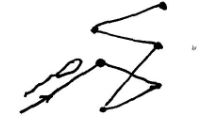
\includegraphics[width=.2\textwidth]{Figures/introduction/runandtumble.png}
    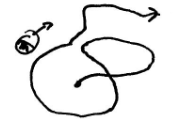
\includegraphics[width=.2\textwidth]{Figures/introduction/smooth.png}
    \caption{Run and tumble versus smooth trajectories of self-propulsion}
    \label{fig: run and tumble vs smooth}
\end{figure}

As a minimal model of active velocity, we can thus simply assume that the particle self-propels at constant speed $v_0$, while the unit vector $\he$ parametrizing its orientation is a colored noise with zero mean and exponential correlations:
\begin{equation} \label{eq_cf_e}
    \langle \he(t) \cdot \he(t + \tau) \rangle = e^{-\tau / \tau_r}.
\end{equation}


We then immediately deduce that, assuming the noise of the orientation and force is independent,
\begin{align}
    \langle |\Delta \bm r(t)|^2 \rangle & = 2 d D t 
    + v_0^2 \int_0^t\rmd\tau_1\int_0^t\rmd\tau_2 \, e^{-|\tau_1-\tau_2|/\tau_r} \nonumber \\
    & = 2 d D t 
    + 2 \lp^2 \left( \frac{t}{\tau_r} - 1 + e^{-t/\tau_r} \right).
\end{align}
%
This has two limiting regimes, much smaller and much larger times than the reorientation time,
%
\begin{align*}
    \langle |\Delta \bm r(t)|^2 \rangle & 
    \underset{t \ll \tau_r}{\simeq} 2 d D t + v_0^2 t^2 , \\
    \langle |\Delta \bm r(t)|^2 \rangle & 
    \underset{t \gg \tau_r}{\simeq} 2 d D_{\rm eff} t , \qquad  D_{\rm eff} = D + \frac{v_0^2\tau_r}{d}. 
\end{align*}
%
This corresponds to three dynamical regimes, with thermal diffusion at short times ($t < 2 d D / v_0^2)$, ballistic dynamics at intermediate times ($2 d D / v_0^2 < t < \tau_r)$ and diffusive motion at long times $t > \tau_r$. 
This confirms the qualitative picture drawn earlier, and is illustrated in \autoref{fig: MSD}.

\begin{figure}[!htb]
    \centering
    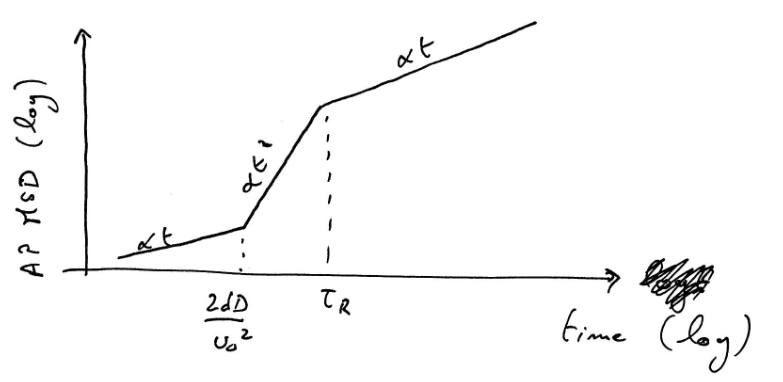
\includegraphics[width=.6\textwidth]{Figures/introduction/crossover.png}
    \caption{The mean-square displacement for different regimes}
    \label{fig: MSD}
\end{figure}






% Handwritten page XIII

\section{Phase transitions and critical phenomena}

Phase transition is a central concept in active matter.
One important example is the flocking transition, where directed units spontaneously choose a direction to align in and move together as a flock.
This is the Active Matter version of the ordering transition in the Ising model, in which spins align in the case of a ferromagnet or anti-align in the case of an anti-ferromagnet.
Here, we will review some basic features of the theories of phase transitions at equilibrium, and introduce tools that we apply in the context of Active matter.



\subsection{A simple example: the Ising model}

One of these important features of phase transitions is that they are associated with the notion of scale-invariance.
A minimal example of this is the Ising model.
Take $N$ spins, $s_i = \pm 1$ on a lattice, whose energy is given by
%
\begin{align}
    E = - \frac{1}{2}J \sum_{\E{ij}} s_i s_j.
\end{align}
%  
Here, $\E{ij}$ indicates that the sum is first over all $i\in\{1...N\}$, then all nearest negihbours $j$ of $i$.
The partition function, a sum over all possible configurations $\{s_i\}$, is
%
\begin{align}
    Z = \sum_{\{s_i\}} e^{-\beta E}.
\end{align}
%
We define the order parameter,
%
\begin{align}
    m = \frac{1}{N}\sum_i s_i,
\end{align}
%
which measures the magnetization.
If all spins points in one direction, then $m  = \pm 1$, while if they are completely randomly distributed, $m = 1$
First, we apply a simple mean-field analysis and assume that the value of each spin is close to that of the average, so $s_i \approx m + \delta s_i$, where $\delta s_i$ is small.
Then,
%
\begin{align}
    s_i  s_j = m^2 + m(\delta s_i + \delta s_j) + \Oh(\delta s^2)
    \approx m(s_i + s_j - m).
\end{align}
%
Here, we have neglected terms that are second order in the perturbations $\delta s$.
% Handwritten page XIV
With this assumption, we may rewrite the energy as
%
\begin{align}
    E_{MF} 
    &= \frac{1}{2} J m \sum_{\E{ij}}(s_i + s_j - m)\\
    & = \frac{1}{2} J m z \left( 2 \sum_{i} s_i - m N  \right).
\end{align}
%
Here, $z$ is the number of nearest neighbors for each site, the coordination number of the lattice.
This depends on the structure of the lattice and the dimensionality in space.
For square lattices, $z = 2 d$, where d is the dimension of space.
Inserting this into the partition function gives
%
\begin{align}
    Z_{MF} & = \sum_{\{s_i\}} \exp \left\{\frac{1}{2}\beta J m z \left( 2\sum_{i} s_i - mN \right) \right\}\\
    & = e^{-\frac{1}{2}\beta J z m^2} 
    \left[\exp \left\{\frac{1}{2}\beta J m z \left( 2\sum_{s=\pm} s \right) \right\}\right]^2\\
    & = e^{-\frac{1}{2}\beta J z m^2} \left[2 \cosh \beta J m z\right]^N.
\end{align}
%
The Helmholtz free energy is given by the logarithm of the partition function, $F = - k_B T \ln Z$, so the mean-field free energy is \todo[noinline]{we should use either $\beta$ or $k_BT$.}
%
\begin{align}
    F_{MF} = N k_B T \left[ \frac{1}{2}\beta Jm^2 z - \ln\left(\cosh \beta J m z\right) \right].
\end{align}
%
The system will, left to its own devices at constant volume and temperature, minimize the free energy.
The magnetization of the system is therefore found by minimizing $F$,
%
\begin{align}
    \pdv{F_{MF}}{m} = 0
    \iff m = \tanh \beta J m z.
\end{align}
%
We may solve this graphically by drawing both functions, as illustrated below.
This shows that for inverse temperatures $\beta = 1 / k_B T$ so that $\beta J z < 1$, there is only one stationary point free energy, $m = 0$.
In this case, this is also a minimum.
For $\beta J z > 1$, there appear two additional stationary $m = \pm m_0$ points.
These are now two degenerate minima of the free energy, while $m = 0$ is a local maximum.
There is thus a \emph{phase transition} at the finite, critical temperature defined by $k_B T_c = J z$.

\begin{figure}[!htb]
    \centering
    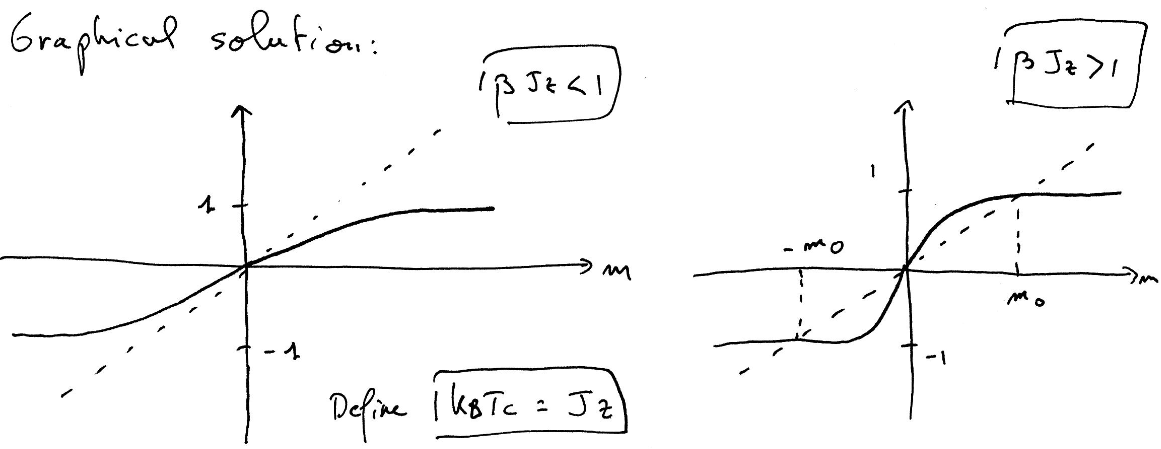
\includegraphics[width=\textwidth]{chapters/Figures/introduction/minimize.png}
    \caption{Minimization for different cases}
    \label{fig: free energy minimization}
\end{figure}

At the phase transition, the $m \rightarrow - m$ symmetry is spontaneously broken, as the magnetization $m$ picks out one of the degenerate minima $m = \pm m_0$.
If we expand the free energy around the point of phase transition $T \approx T_c$ where $m$ is small, we get
%
\begin{align}
    F_{MF}
    \sim 
    \frac{1}{2} Nk_B TC
    \left[
        \left(\frac{T - T_c}{T} m^2 + \frac{T_c}{T} \frac{m^4}{6}\right)
    \right]
    + \Oh(m^6).
\end{align}
%
This is the \emph{Landau Free energy}.
With the reduced temperature $t = (T - T_c) / T_c$, often called the control parameter, t has the form $F = \frac{1}{2} \alpha t m^2 + \beta \frac{1}{4} m^4$.
As the $m^2$ changes sign at $t = 0$, this free energy goes from a single-well potential to a double-well one.
This is a characteristic feature of phase transitions.

\begin{figure}[!htb]
    \centering
    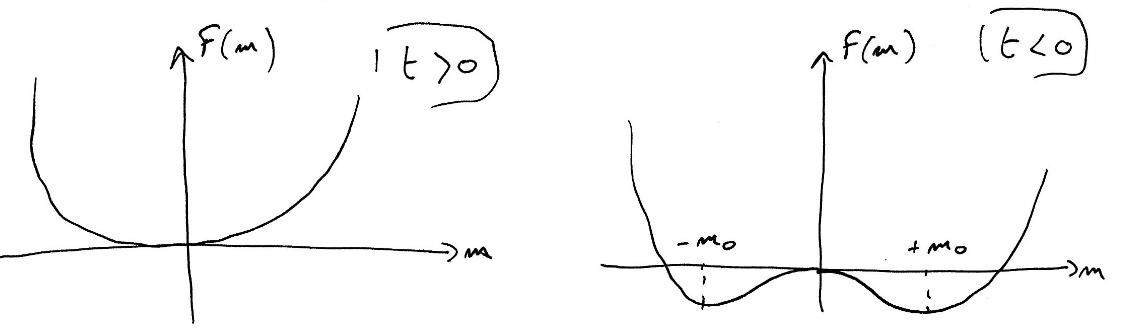
\includegraphics[width=.8\textwidth]{chapters/Figures/introduction/double_well.png}
    \caption{The double Landau free energy changes from a single to a double well as the control parameter is tuned past the critical point.}
    \label{fig: double well}
\end{figure}

To go beyond the mean-field approach, we include spatial dynamics.
This means that the magnetization field now depends on space, $m = m(\bm x)$.
We assume the free energy density has the same Landau form close to the critical temperature, 
%
\begin{align}
    f(m) = \frac{1}{2}\alpha t  m^2 + \frac{1}{4} \beta m^4,
\end{align}
%
where $\alpha \approx N K_B T_c$ and $\beta \approx N k_B T_C / 3 \approx \alpha / 3 $. \todo[noinline]{shoudl we not divide out $N$ to get an intensive quantity?}
This is the ``Bulk free energy density''.
The full free energy is the integral of this density, plus a term that takes into account the cost of gradients.
The lowest order term which is invariant under spatial orientations, which we must have as this is a symmetry of the microscopic dynamics, is $|\nabla m|^2$.
Combining these terms together gives us the Ginzburg-Landau free energy functional\footnote{\emph{Functional}, not function, as this is a function of a function $m(\bm x)$. This means derivatives $\odv{}{m}$ now becomes functional derivatives, $\fdv{}{m(\bm x)}$.}
%
\begin{align}
    F[m] = \int \dd \bm x 
    \left(f(m) + \frac{1}{2} K |\nabla m|^2\right).
\end{align}
%


To obtain a dynamical equation for this system, which governs the time-evolution of $m$, we assume pureyly dissipative dynamics, 
%
\begin{align}
    \pdv{}{t} m(\bm x, t)
    =
    \fdv{F}{{M(\bm x, t)}} 
    = - [\alpha t + \beta m(\bm x, t)] m(\bm x, t) + K \nabla^2 m^2.
\end{align}
%
If we assume a homogeneous configuration $m = m_0$, where $\nabla m_0 = 0$, the steady state solution is
%
\begin{align}
    (\alpha t + \beta m_0^2) m_0 = 0
    \implies
    \begin{cases}
        m_0 = 0, & t > 0, \\
        m_0 = \sqrt{ \frac{ \alpha |t| }{ \beta } }, & t < 0,
    \end{cases}
\end{align}
%
as before.
However, we may now also consider how this state responds to fluctuation.
We write $m(\bm x, t) = m_0 + \delta m(\bm x, t)$, and study the dynamics of $\delta m$ at linear level.
The equation of motion is
%
\begin{align}
    \pdv{}{t} \delta m = - a^2 \delta m  + K \nabla^2 \delta m + \xi,
\end{align}
%
where
%
\begin{align}
    a = 
    \begin{cases}
        \alpha t, & t > 0, \\
        2 \alpha |t|, & t < 0,
    \end{cases}
\end{align}
%
and $\xi$ is Gaussian white noise, satisfying
%
\begin{align}
    \E{\xi(\bm x, t)} &= 0, &
    \E{\xi(\bm x, t) \xi(\bm x', t')}
    = \Xi \delta^d(\bm x - \bm x') \delta(t - t').
\end{align}
%
We consider the equations in Fourier space by inserting the fourier transform of the perturbation,
%
\begin{align}
    \delta \hat m(\bm q, \omega)
    =
    \int \dd \bm x \dd t \, e^{i(\bm q \cdot \bm r + \omega t)} \delta m(\bm x, t),
\end{align}
%
which gives
%
\begin{align}
    (i \omega + a^2 + Kq^2)\delta \hat m = \hat \xi(\bm q, \omega).
\end{align}
%
The Fourier transform of the noise also has vanishing expectation value and the covariance
%
\begin{align}
    \E{\hat \xi(\bm q, \omega)\hat\xi(\bm q', \bm \omega')}
    = \Xi (2\pi)^{d + 2}\delta^d(\bm q + \bm q') \delta(\omega + \omega').
\end{align}
%
With this, we easily can explicitly calculate the Fourier transform of the two-point correlation function,
%
\begin{align}
    \hat C(\bm q, \bm \omega)
    = 
    \frac{\E{\delta \hat m(\bm q, \omega) \delta \hat m(\bm q', \omega')}}{(2\pi)^{d + 2}\delta^d(\bm q + \bm q') \delta(\omega + \omega')  }
    = 
    \frac{\Xi}{\omega^2 + (a^2 + K q^2)^2}.
\end{align}
%
We obtain the equal-time correlation by integrating over frequency space, corresponding to the Fourier-transform at $t = 0$, which we can perform by contour integration \todo[noinline]{Draw contour, explain}
%
\begin{align}
    \hat C(\bm q) = \int \frac{\dd \omega}{2 \pi} \hat C(\bm q, \omega)
    = 
    \frac{1}{2}\frac{\Xi }{a^2 + K q^2}.
\end{align}
%
In real space, the two-point function is
%
\begin{align}
    C(\bm x)
    = \E{\delta m(0) \delta m(\bm x)}
    = \frac{\Xi}{2 K}
    \int \frac{\dd \bm q}{(2 \pi)^d} \frac{e^{-i\bm q \cdot \bm x}}{\xi^{-2} + q^2},
\end{align}
%
where we have introduced the \emph{correlation length}
%
\begin{align}
    \xi = \sqrt{ \frac{ K }{ a^2 } }.
\end{align}
%
The two-point function measures how correlated the magnetization at two different spatial points, separated by $\bm x$, are.
The correlation length $\xi$ is the length scale over which this correlation is significant.
We may see this by taking the two limits of the integral
%
\begin{align}
    C(r) = 
    \begin{cases}
        \frac{1}{r^{\frac{d - 2}{2}}} e^{- r / \xi}, & r \gg \xi, \\
        \frac{1}{r^{d - 2}}, & r \ll \xi.
    \end{cases}
\end{align}
%
Thus, for distances less than the correlation length, the correlation falls off algebraically, $C \sim r^{2 - d}$, while at longer distances it is exponentially suppressed.
In other words, when $\xi \sim \sqrt{ |t| }$ is finite, spins are correlated at a scale $\xi$.
When we approach the critical point $t \rightarrow 0$, the correlation length diverges and the systems becomes \emph{scale free}.

At the critical point, the physics is independent of the microscopic details of the dynamics.
The large-scale behavior of the system is set by the correlation length, which may be arbitrarily large.
These are the ideas at the root of the powerful concept of \emph{universality} in physics.
At a critical point, the only thing that governs the physics of a system is its characteristics like the symmetries, conservation laws and dimensionality, placing it in its universality group, not the specific of the microscopic equation of motion.

A critical point is characterized by a set of critical exponents, which governs how measurable quantities scales with the control parameter.
Examples are
%
\begin{align}
    |m_0| &\sim |t|^\beta, &
    \xi & \sim |t|^{-\nu}, &
    C(r) & \sim r^{d - 2 + \eta}.
\end{align}
%
However, the mean-field predictions that we obtained earlier for these exponents are generally incorrect, because we have neglected the non-linearities in the equation, and we have not taken into account the effects of fluctuations.
In fact, the one-dimensional Ising model can be solved exactly, and \emph{does not} feature a phase transition at finite temperature.
In one dimension, there are too few nearest neighbors to keep spins ordered when thermal noise is introduced, and any non-zero temperature results in a finite correlation length.

In the case of the Ising model, the mean-field breaks down for all dimensions lower than its \emph{critical dimension}, $d < d_c = 4$.
To go beyond the mean field prediction and obtain accurate results for the critical exponents, one has to employ the \emph{Renormalization Group} or RG for short.
In this method, one explicitly integrates out the short-wavelength dynamics.
With this, one may derive equations describing how the parameters in the free energy, such as $\alpha$ and $\beta$ above, change as one changes the scale of the theory.
These are the \emph{Renormalizatio Group Equations}.
A fixed point in the RG equations means that the parameters do not change, and thus that the corresponding model is scale-free.
Below we report some of the exponents for the Ising model.
In 2 dimensions, the Ising model was solved by Lars Onsager in 1944.
This allows for the computation of exact exponents.
In 3 dimensions, one has to resort to renormalization or numerics.
In the table below, we provide some the exponents in various dimensions.
Thos in 2D are exact, the 3D ones are from numerics, while those above 4D are the mean-field exponents.

\begin{table}[h]
    \centering
    \begin{tabular}{r|c c c}
        $d$ & 2 & 3 & >4 \\
        \hline
        $\beta$ & $1/8$ & $0.3264$ & $1 / 2$ \\
        $\nu$ & $1$ & $0.6300$ & $1 / 2$ \\
        $\eta$ & $1/4$ & $0.363$ & $0$
    \end{tabular}        
\end{table}


\subsection{Continuous symmetry breaking: Goldstone modes and the Mermin-Wagner theorem}


Similar ideas also hold for systems out-of-equilibrium when scale-free behavior is present.
This motivates the classification of active systems in terms of their conservation laws and symmetries.
The Ising model has the discrete symmetry $s_i \rightarrow -s_i$, in mathematical terms $\mathbb{Z}_2$.
The equations of motion, and thus all physics, remain unchanged if all spins are flipped upside-down.
We will now consider spins that are free to rotate around, and not just point up or down so that the spin at each site is represented by a vector $\bm s_i$.
The corresponding magnetization is also a vector, 
%
\begin{align}
    \bm m = \frac{ 1 }{ N } \E{{\sum}_i \bm s_i}.
\end{align}
%
We still consider the nearest-neighbor interactions, so the energy is
%
\begin{align}
    E = - \frac{1}{2}J \sum_{\E{ij}} \bm s_i \cdot \bm s_j.
\end{align}
%
This energy is invariant under the rotation of all the spins at the same time.
This symmetry, which in group theory is called a $\mathrm{O}(N)$ symmetry where $N$ is the number of dimensions of the vector being rotated, is continuous.

If we take the Ginzburg-Landau approach, we may write down a low-order expansion of the free energy which is invariant under $ \mathrm{O}(N)$, 
%
\begin{align}
    F = \int \dd \bm x \, 
    \left(
        \frac{1}{2} t |m|^2 + \frac{1}{4} |m|^4 + \frac{1}{2} K |\nabla m|^2
    \right)
\end{align}
%
This free energy has the famous Mexican-hat shape, illustrated below.

\begin{figure}[!htb]
    \centering
    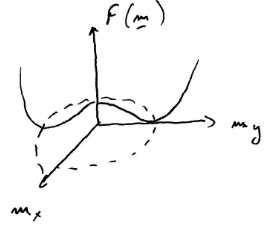
\includegraphics[width=.4\textwidth]{chapters/Figures/introduction/mexican.png}
    \caption{The Mexican-hat potential.}
    \label{fig: mexican}
\end{figure}

Here, the gradient term represents a dot-product of both the gradients and the magnetization, $|\nabla m|^2 = \nabla_\alpha m_\beta \nabla_\alpha m_\beta$.
We now follow the same procedure, leading to the dynamics,
%
\begin{align}
    \partial_t \bm m = - (t + |m|^2) \bm m + K \nabla^2 \bm m,
\end{align}
%
and the steady-state solution
%
\begin{align}
    |m|^2 = 
    |m_0|^2 
    =
    \begin{cases}
        0, & t > 0 \\
        |t|, & t < 0 
    \end{cases}
\end{align}
%
Now, the steady-state solution is picked not from two degenerate minima, but instead from a continuum of degenerate minima.
The minimizing solution has the form $\bm m_0 = m_0 \hat {\bm u}_\parallel$, where $\hat {\bm u}_\parallel$ is a unit vector spontaneously breaking the rotational symmetry by pointing out a direction int $\bm m$-space.

We then perform a linear perturbation, bu now we must write
%
\begin{align}
    \bm m &= (m_0 + \delta m_\parallel) \hat {\bm u}_\parallel + \delta \bm m_\perp, &
    \delta \bm m_\perp \cdot \hat {\bm u}_\parallel &= 0.
\end{align}
%
We consider the case where $m_0 = 0$, i.e., $t < 0$.
The equations of the perturbations, at linear order, is
%
\begin{align}
    \partial_t \delta m_\parallel 
    & = 
    2 t \delta m_\parallel + K \nabla^2 \delta m_\parallel + \xi_\parallel, \\
    \partial_t \delta \bm m_\perp
    & = K \nabla^2 \delta \bm m_\perp + \xi_\perp.
\end{align}
%
We see that $\delta m_\parallel$ follows a similar equation as for the Ising model, with a correlation length $\xi = \sqrt{ K / 2 |t| }$, while for $\delta \bm m_\perp$ there is seemingly no correlation length.
$\delta \bm m_\perp$ is therefore a \emph{Goldstone mode}, with infinite correlation.
In the language of high-energy physics, the modes are massless.
This results from the spontaneous breaking of a continuous symmetry.
When this happens, there is no energetic cost associated with a global rotation.
Consider the Mexican hat, given some direction of symmetry breaking, one can always rotate the corresponding unit vector around the center without incurring an energetic cost.

This, furthermore, implies that the corresponding two-point same-time correlation functions, in Fourier space, have the form
%
\begin{align}
    \hat C(\bm q) = (d - 1)\frac{\eta_\perp}{2 K q^2}.
\end{align}
%
The corresponding real-space correlation functions quantify the typical amplitude of thermal fluctuations.
By imposing a Lattice size, $a$ and a system size $L$, we get finite limits for our integral and consider the dominant behavior as we approach a continuous system, $a \rightarrow 0$, in the thermodynamic limit, $L \rightarrow \infty$,
%
\begin{align}
    \E{|\delta(\bm x)|^2} = \int \frac{\dd\bm q}{(2 \pi)^d} 
    \propto \int_{1 / L}^{1/a} q^{d - 3}
    \sim
    \begin{cases}
        L^{2 - d}, & d < 2, \\
        \ln\frac{L}{a}, & d = 2, \\
        a^{2 - d}, & d > 2.
    \end{cases}
\end{align}
%
For $d > 0$, the fluctuations diverge as the lattice spacing goes to zero.
These are called ultra-violet (UV) divergences because they are divergences due to dynamics at short wave lengths, which for light is the ultra-violet part of the spectrum.
No statistical-mechanical system, however, has infinitely small units, there is always some small wave-length for which the field theory description breaks down.
This divergence is therefore unphysical, and something we have to regularize our theory to deal with.
For $d < 2$, however, the fluctuations diverge in the thermodynamic limit where the system size becomes infinite.
These are called infra-red (IR) divergences, as they are due to the large-wavelength dynamics.
This is exactly the regime where we are hoping our model is a good description and not something we can sweep under the rug.
In $d = 2$, the lower critical dimension for the $\mathrm{O}(N)$ model, the theory diverges both in the IR and the UV.

The IR divergence is a physical prediction.
What it tells us is that our assumption of a state that is mostly ordered, with small fluctuations $\bm m = \bm m_0 + \delta \bm m $ is wrong.
In fact, for $d \leq 2$, there cannot be long-range order.
This is an instance of the \emph{Mermin-Wagner theorem}, which states that there cannot be spontaneous breaking of a continuous symmetry in dimension $d = 2$ or lower.
